\newcommand{\lecturetitle}{Convolutional Neural Networks III}
\newcommand{\lecturesubtitle}{Implementation, diagnosis, features, and transfer}
\newcommand{\covertext}{Build\\inspect\\adapt}

% Shared preamble for new AICE3002/AICE6001 lecture decks.
% Define \lecturetitle, \lecturesubtitle and \covertext before including this file.

\ifdefined\beamerclass
\else
  \def\beamerclass{beamer}
\fi

\ifdefined\articlemode
  \documentclass[]{article}
  \usepackage[a4paper,margin=2cm]{geometry}
  \usepackage[envcountsect]{beamerarticle}
  \usepackage{parskip}
  \usepackage[hidelinks]{hyperref}
\else
  \documentclass[\beamerclass,ignorenonframetext]{beamer}
\fi

\usepackage{pgfpages}
\mode<handout>{
  \pgfpagesuselayout{2 on 1}[a4paper,border shrink=5mm]
}

\usepackage{lmodern}
\usepackage[english]{babel}
\usepackage[utf8]{inputenc}
\usepackage{amsmath}
\usepackage{bm}
\usepackage{graphicx}
\usepackage{hyperref}
\usepackage{tikz}

\usetheme{Copenhagen}
\useoutertheme{infolines}
\setbeamertemplate{headline}{}
\setbeamertemplate{navigation symbols}{}
\hypersetup{pdfstartview={Fit}}

\definecolor{darkblue}{RGB}{37,55,97}
\definecolor{mellowyellow}{RGB}{247,206,70}

\title[AICE3002 / AICE6001]{\lecturetitle}
\subtitle{\lecturesubtitle}
\author{Jonathon Hare}
\institute[]{
  Vision, Learning and Control\\
  University of Southampton
}
\date{}
\subject{Computer Science}

\begin{document}
\mode<article>{\maketitle}

\mode<presentation>{
  \begin{frame}[plain]
    \begin{tikzpicture}[
      overlay,
      remember picture,
      shift={(current page.south west)},
      font={\fontfamily{Montserrat-TOsF}\selectfont}
    ]
      \fill[mellowyellow] (0,0) rectangle (\paperwidth,\paperheight);
      \node[
        anchor=west,
        align=left,
        text=darkblue
      ] at (1.5,5.6) {\Huge\bfseries \begin{tabular}{l}\covertext\end{tabular}};
      \node[anchor=west,text=darkblue] at (1.5,1.1) {\large AICE3002 / AICE6001};
      \node[anchor=east] at (12.3,1.0) {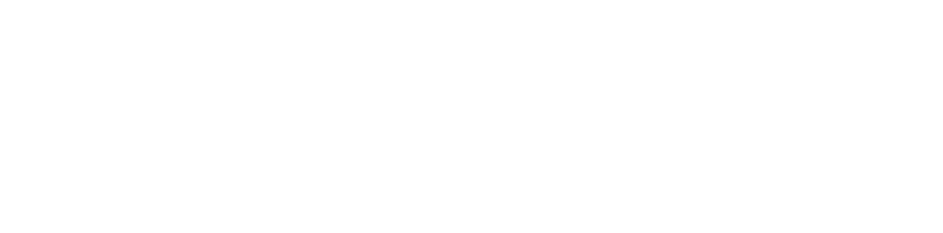
\includegraphics[scale=0.15]{../vlc.png}};
    \end{tikzpicture}
  \end{frame}
}

\begin{frame}
  \titlepage
\end{frame}


\frame{\frametitle{Turning an architecture diagram into code}}
\frame{\frametitle{Tracking tensor shapes through a CNN}}
\frame{\frametitle{Checking parameter counts and receptive fields}}
\frame{\frametitle{Feature hierarchies emerge across depth}}
\frame{\frametitle{Visualising activations and filters}}
\frame{\frametitle{Diagnosing optimisation and generalisation failures}}
\frame{\frametitle{What a pretrained representation provides}}
\frame{\frametitle{Feature extraction versus fine-tuning}}
\frame{\frametitle{Designing a controlled architecture comparison}}
\frame{\frametitle{Separating architectural gains from training gains}}
\frame{\frametitle{A practical CNN investigation}}

\end{document}
